\documentclass{article}    

\usepackage{graphicx}

\begin{document}

% ------------------------------------------ figure 13

\begin{figure*}[!ht] \centering
  \begin{tabular}{cc}
    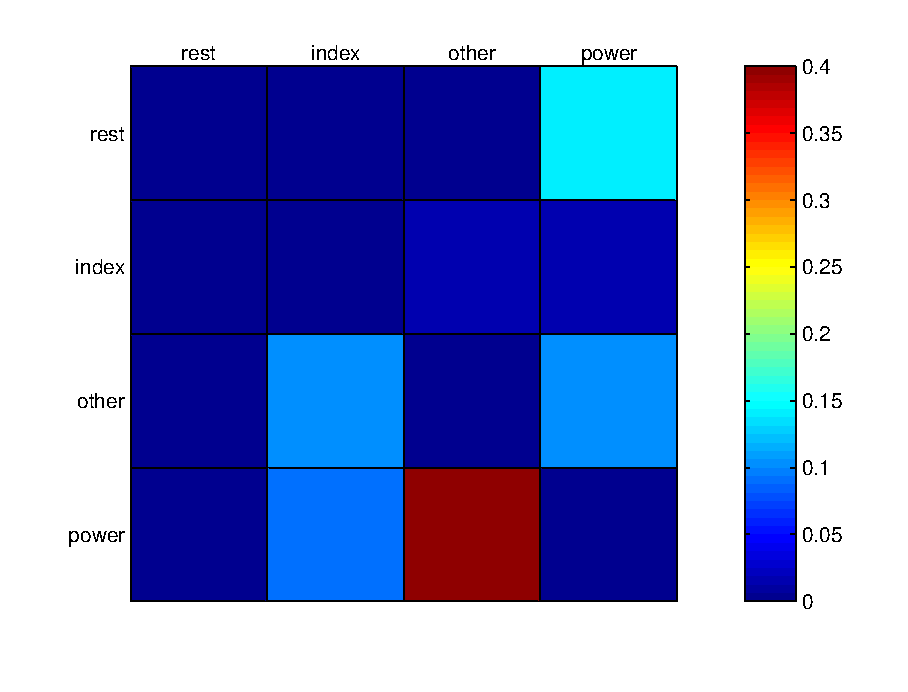
\includegraphics[width=0.45\textwidth]{confMat_1.eps} &
    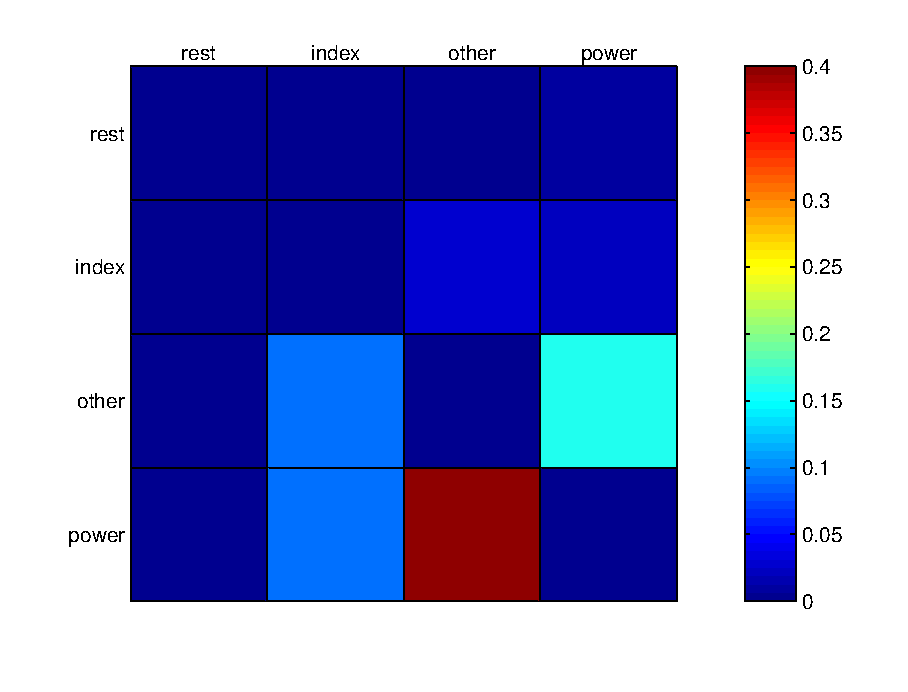
\includegraphics[width=0.45\textwidth]{confMat_2.eps} \\
  \end{tabular}
%  \caption{confusion matrices for the SA phase (left) and FA phase (right). Each matrix
%           is the average over the confusion matrices of the $10$ subjects. A confusion
%           matrix $C$ is such that its $(i,j)$th element is the fraction of $i$ labels
%           mistaken for $j$ labels, over the total mistaken labels.}
%  \label{fig:confusion}
\end{figure*}

\end{document}
